\documentclass[conference]{IEEEtran}
\IEEEoverridecommandlockouts
% The preceding line is only needed to identify funding in the first footnote. If that is unneeded, please comment it out.
\usepackage{cite}
\usepackage{amsmath,amssymb,amsfonts}
\usepackage{algorithmic}
\usepackage{graphicx}
\usepackage{textcomp}
\usepackage{xcolor}
\usepackage{hyperref}
\usepackage[ngerman]{babel}

\def\BibTeX{{\rm B\kern-.05em{\sc i\kern-.025em b}\kern-.08em
    T\kern-.1667em\lower.7ex\hbox{E}\kern-.125emX}}
\begin{document}

\title{Augmented Reality in Education
}

\author{\IEEEauthorblockN{Tobias Wen Klingenberg}
\IEEEauthorblockA{\textit{School of Computation, Information and Technology} \\
\textit{Technische Universität München}\\
München, Deutschland \\
t.klingenberg@tum.de}
}
\maketitle

\begin{abstract}
Innovation in der Bildung ist seit jeher eine erstrebenswerte, aber meißt nicht
vorhandene oder durchsetzbare Thematik die in den letzten Jahren immer mehr 
Aufmerksamkeit bekommen hat. Eine dieser Innovationen ist die Augmented Reality
(Erweiterte Realität), welche tatsächlich sehr sinnvolle und bereichernde 
Möglichkeiten für die Bildung bieten kann.
Das folgende Paper befasst sich mit der Entwicklung, 
Anwendung und Analyse der Möglichkeiten von Augmented Reality 
in der Bildung.
\end{abstract}

\section{Einleitung}
Augmented Reality (im Folgenden AR) ist eine Innovation, welche in den letzten
Jahren immer mehr Akzeptanz und tatsächliche Anwendung in unserem täglichen
Leben genießen konnte. Sie ist eine Technologie, welche es ermöglicht, digitale
Informationen mit der echten physischen Welt zu überlagern und somit die persönliche 
Sicht ''erweitern''.

Dazu gibt es verschiedenste Innovationen, die dieses Konzept 
auf unterschiedlicher Weise ermöglichen. Durch diese Verschmelzung
der digitalen und realen Welt eröffnen sich vollkommen neue Anwendungsmöglichkeiten
, wie unter anderem interaktive Lernumgebungen, Unterstützung im medizinischen Bereich
oder Unterhaltungs- und Unterstützungsmedien. Im Folgenden wird vor allem auf die möglichen 
Anwendungen im Bildungsbereich eingegangen.


\section{Motivation}

AR bietet sich vor allem aus mehreren Gründen für eine Anwendung in den verschiedensten
Bildungsmöglichkeiten an. Dazu gehört vor allem eine stärkere Gedächtnisleistung aufgrund von
visuellen und interaktiven Inhalten, sowie ein personalisiertes Lernen durch Anpassung 
auf individuell nötigen Bedürfnissen. \cite{b1} 

Eine hohe Motivation unter den Schüler:innen 
kann mit Ansätzen einer spielerischen Bildung ermöglicht werden. Vor allem interssant ist 
die mögliche kontextualisierte Lernerfahrung, indem theoretisches Wissen in simulierten 
Umgebungen angewedent werden kann. \cite{b2} TODO

\section{Entwicklung}
In den vergangen Jahren ließ sich eine immer höhrer Nachfrage für AR Technologien im Bildungsbereich
feststellen. Vor allem in der Forschung ist dieser Trend sichtbar, in der tatsächlichen Anwendung ist die
Adaption von diesen Technologien zwar vorhanden, jedoch noch immer nicht weitverbreitet. \cite{b3}

In Abb. \ref{fig1} lässt sich die Entwicklung des Themas Bildung mit AR darstellen. Die Abbildung zeigt die Anzahl
der veröffentlichten Paper in diesem Bereich von 2014 bis 2020 \cite{w2}. Ein klarer Sprung lässt sich in dem Jahr 2014 feststellen,
in welchem die Google Glasses vorgestellt wurden. Diese ermöglichten eine tatsächliche konsumentenorientiertete 
Möglichkeit, AR selbst umzusetzen. Dadurch wurde die Forschungsintensität in diesem Bereich verstärkt. 
Ein ähnlicher Sprung lässt sich im Jahr 2020 erkennen, welcher wohlmöglich aufgrund der Covid-19 Pandemie einen
Forschungsschwerpunkt in Richtung von Remote Unterricht als Grund hat.

\begin{figure}[htbp]
    \centerline{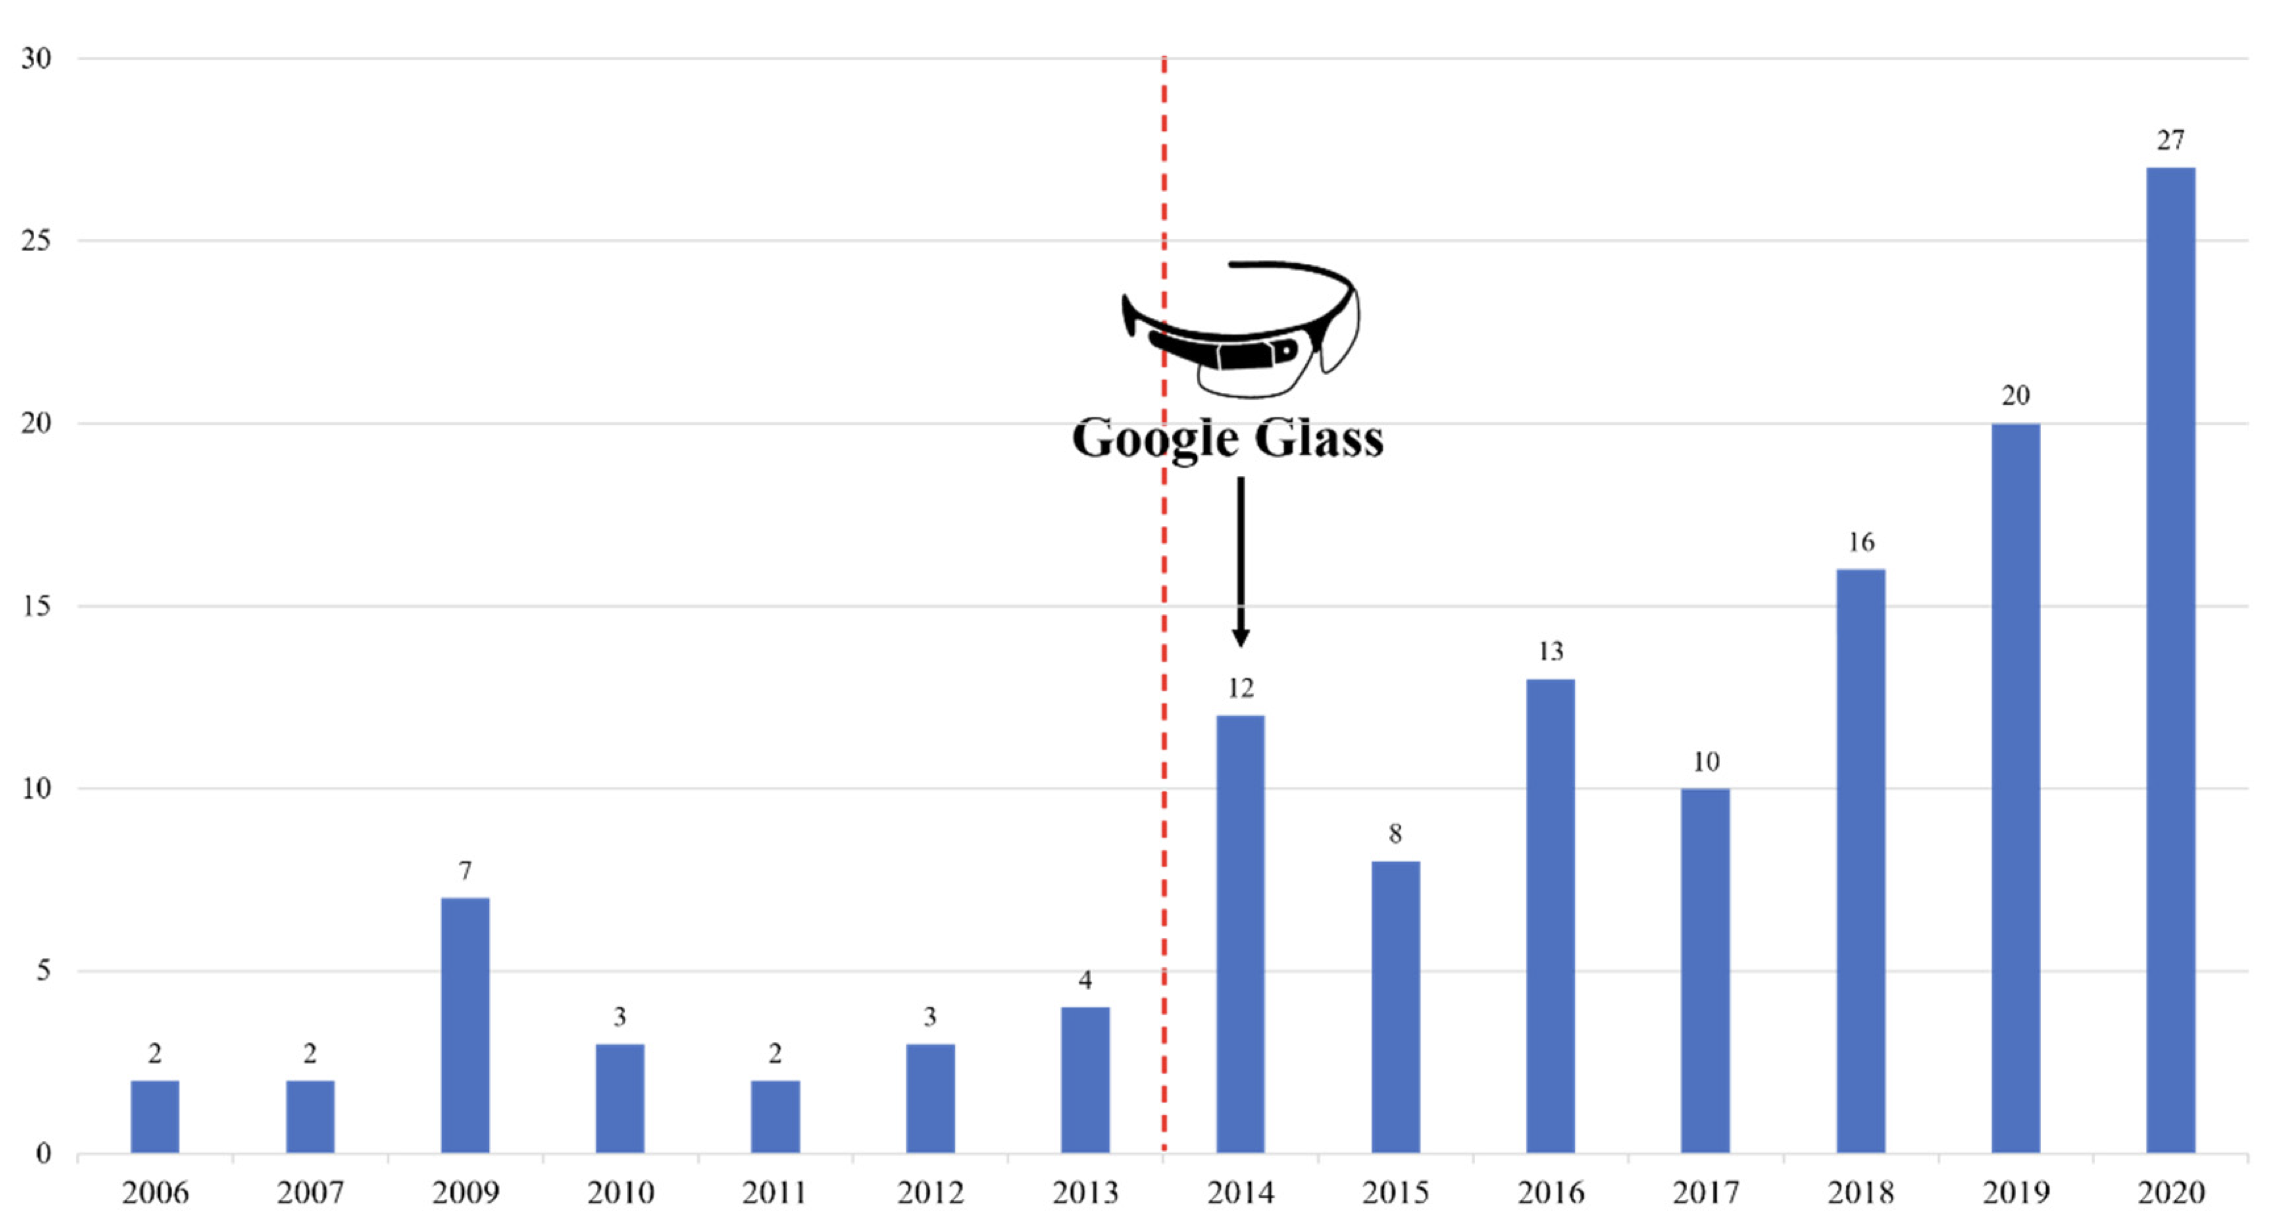
\includegraphics[scale=0.2]{img/entwicklung.png}}
    \caption{Anzahl an Paper über AR in der Bildung}
    \label{fig1}
\end{figure}

\section{Tools und Plattformen}\label{AA}
Damit AR in der Bildung funktionieren kann, müssen einige Kriterien erfüllt sein. Das Zusammenspiel
zwischen Software und Hardware ist essenziel um eine immersive und interaktive Lernerfahrung
zu ermöglichen. Moderne Software ermöglicht es, Laborexperimente oder geschichtliche Ausflüge
zu veranstalten. Damit dies nahtlos in den Unterricht integriert werden kann, ist es wichtig, passende
Hardware zu unterstützen.
Im folgenden werden auf diese eingegangen und an einigen realen Beispielen diskutiert.

\subsection{Software}
Damit die Software in den Bildungssektor passt, müssen Kriterien wie eine einfache Bedienung,
weite Verbreitung, kostengünstig und passenden Inhalt gewährleistet sein. Momentan
vorhandene Beispiele sind unter anderem:
\begin{itemize}
    \item \href{https://sites.google.com/dublinschools.net/vr-ar/google-geo-tools/google-expeditions}{Google Expeditions}
    \item \href{https://koerber-stiftung.de/projekte/eustory/teaching-and-learning-in-the-metaverse/}{Metaverse}
    \item \href{https://www.4danatomy.com/}{Anatomy 4D}
    \item \href{https://www.labster.com/}{Labster}
    \item \href{https://www.cospaces.io/}{CoSpaces Edu}
\end{itemize}
Jedes dieser Beispiele fokussiert isch auf einen speziellen Fachbereich
in der Bildung. Während Google Expeditions sich auf virtuelle sowie augmentierte
Erlebnisse und Ausflüge fokussiert, passt sich unter anderem Anatomy 4D speziell
auf die Lehre der Biologie im Bereich Anatomie von Mensch und Tier ab. 
Labster ermöglicht es, teilweise Laborumgebungen zu augmentieren und so völlig neue
Lernumgebungen zu schaffen. Mithilfe von CoSpaces Edu lässt sich unter anderem
das Zusammenarbeiten trotz Distanz ermöglichen, indem andere Personen und Räume in 
den eigenen augmentiert werden können. \cite{w1}

\subsection{Hardware}
Damit die Hardware in den Bereich Bildung passt, muss auf einige Kriterien geachtet werden.
Unter anderem sollte, vor allem in der Benutzung im primären Bildungssektor, auf eine günstige
Hardwareoption geachtet werden. Diese sollte einfach zu bedienen sein und nicht zu zerbrechlich sein.
In der Schule sind für diese Anwendung vor allem bereits vorhandene Hardware zu betrachten, zum Beispiel
LiDAR fähige Tablets sowie Smartphones und Computer die im Sinne der Schule bereits in das Curriculum
integriert sind. Diese benötigen teils keine weiteren Anschaffungskosten und auch keine weitere Schulung und
Weiterbildung der Lehrkräfte und Schüler.

Im Hinblick auf Bildung in der Hochschule und Weiterbildung in der Industrie sind vor allem kostenintesivere,
aber auch immersivere Hardwareoptionen möglich. Darunter gehöhren AR-Brillen und Headsets im Sinne von HUP (Head-up-Display),
Optical see through und Visual see through. Desweiteren gibt es speziell auf Bildung angepasste Hardware wie der 
\href{https://mergeedu.com/cube?cr=4646}{Merge Cube}, welcher es ermöglicht Schülern 3 dimensionale Objekte in der Hand zu
halten und damit zu interagieren. \href{https://zspace.com/}{ZSpace} hingegen ermöglicht es, dem Anwender mithilfe eines Stylus 
ähnlichen Stiftes, Objekte aus dem Monitor zu ziehen und dieses zu manipulieren.

Zu den wichtigsten Beispielen gehören unter anderem:
\begin{itemize}
    \item \href{https://www.microsoft.com/de-de/hololens}{Microsoft HoloLens}
    \item \href{https://www.meta.com/de/quest/quest-3/}{Meta Quest 3}
    \item \href{https://www.apple.com/de/apple-vision-pro/}{Apple Vision Pro}
\end{itemize}

Während das Microsoft HoloLens auf Optical see through setzt, benutzen beide anderen Beispiel Video see through, durch welche
zwar immersivere Erlebnisse gestaltbar sind, jedoch auch Nachteile durch Übelkeit möglich sind.


\section{Virtuelle Räume}
Gerade seit der Covid-19 Pandemie ist auch das Theme der virtuellen Klassenräume interessant geworden.
Dabei ist zu Unterscheiden zwischen dem virtuelle Klassenraum vor Ort und dem von anderen Orten aus.
Das Konzept besteht darin, dass entweder der Klassenraum an sich durch AR erweitert wird und somit der Unterricht
immersiv berreichert wird und, dass der Klassenraum vollkommen in einen anderen Raum augmentiert wird und somit
ein authentischer Unterricht von anderen Orten möglich ist.

\subsection{vor Ort}
Die klassiche und intuitive Art, AR in den Klassenraum einzubauen ist die Art der Anwendung vor Ort.
Der Zweck eines virtuellen Klassenraumes vor Ort besteht darin, dass gemeinsam in Präsenz die Nutzung von AR Hardware in den 
bestehenden Unterricht eingebaut wird. Dies kann in unterschiedlicher Weise genutzt werden. Dazu gehört die Funktionsweise 
als unterstützende Aufgabe während des Unterrichtes. Das momentan besprochene Thema kann durch Simulationen und Rendering von 
Modellen visualisiert werden. Des weiteren können parallel kleinere Aufgaben in Form von spielerischen Ansätzen veranstaltet werden,
um die Motivation und Gedächtnisleistung während des Unterrichts anzuregen. 
\subsubsection*{Probleme}
Zu den hier vorhandenen Problemen gehören vor allem, die hohen Anschaffungskosten, die in vielen Schulsystemen nicht gerechtfertigt
werden können, sowie eine nötige Schulung des entsprechenden Personal. Zum Vergleich, eine Microsoft HoloLens 2 kostet für Bildungseinrichtungen
pro Exemplar rund \href{https://techcommunity.microsoft.com/t5/mixed-reality-blog/education-institutions-save-10-on-microsoft-hololens-2/ba-p/3282493}{3,500\$}
eine Meta Quest 3 rund \href{https://www.meta.com/de/en/quest/quest-3/#}{500\$}, wobei es teilweise Abonnements gibt die dies vergünstigen
können.
\subsection{Remote}
Im Gegensatz zu der Nutzung vor Ort, bietet die Nutzung von AR von Zuhause oder anderen Orten (Remote) einige interessante Ansätze 
und Vorteile. Die Remote Nutzung beinhaltet vor allem das augmentieren einzelner Personen oder ganzer Räume in einen anderen, lokal
gelegenen Raum \cite{b5}. Dies ermöglicht es, Fernunterricht, zum Beispiel aufgrund von einer Quarantäne (individuell oder pandemisch bedingt)
oder aufgrund unzureichend vorhandener Infrastruktur (dazu gehören nicht genug vorhandene Schulen in abgelegenen Gebieten, sowie 
beeinträchtigte Wege). Dabei können Lehrer, optional Mitschüler und jegliche Unterrichtsmaterialien in seinen eigenen Raum 
augmentiert werden, um ein lebendieges und authentisches Lernerlebnis auch außerhalb des Klassenraumes zu ermöglichen
\subsubsection*{Probleme}
Neben den auch hier sehr hohen Investitions- und Schulungskosten, kommt das Problem dazu, dass diese Technologie noch nicht in einer 
anwendbaren Phase entwickelt wurde. Dazu gehört das Echtzeit Scannen von Personen und ganzen Räumen, sowie die Projektion in nicht
vordefinierte Räume.

\section{Anwendungen}
Der Bereich AR in der Bildung lässt sich in 7 Bereiche einteilen (siehe Abb. \ref{fig2}).

\begin{figure}[htbp]
    \centerline{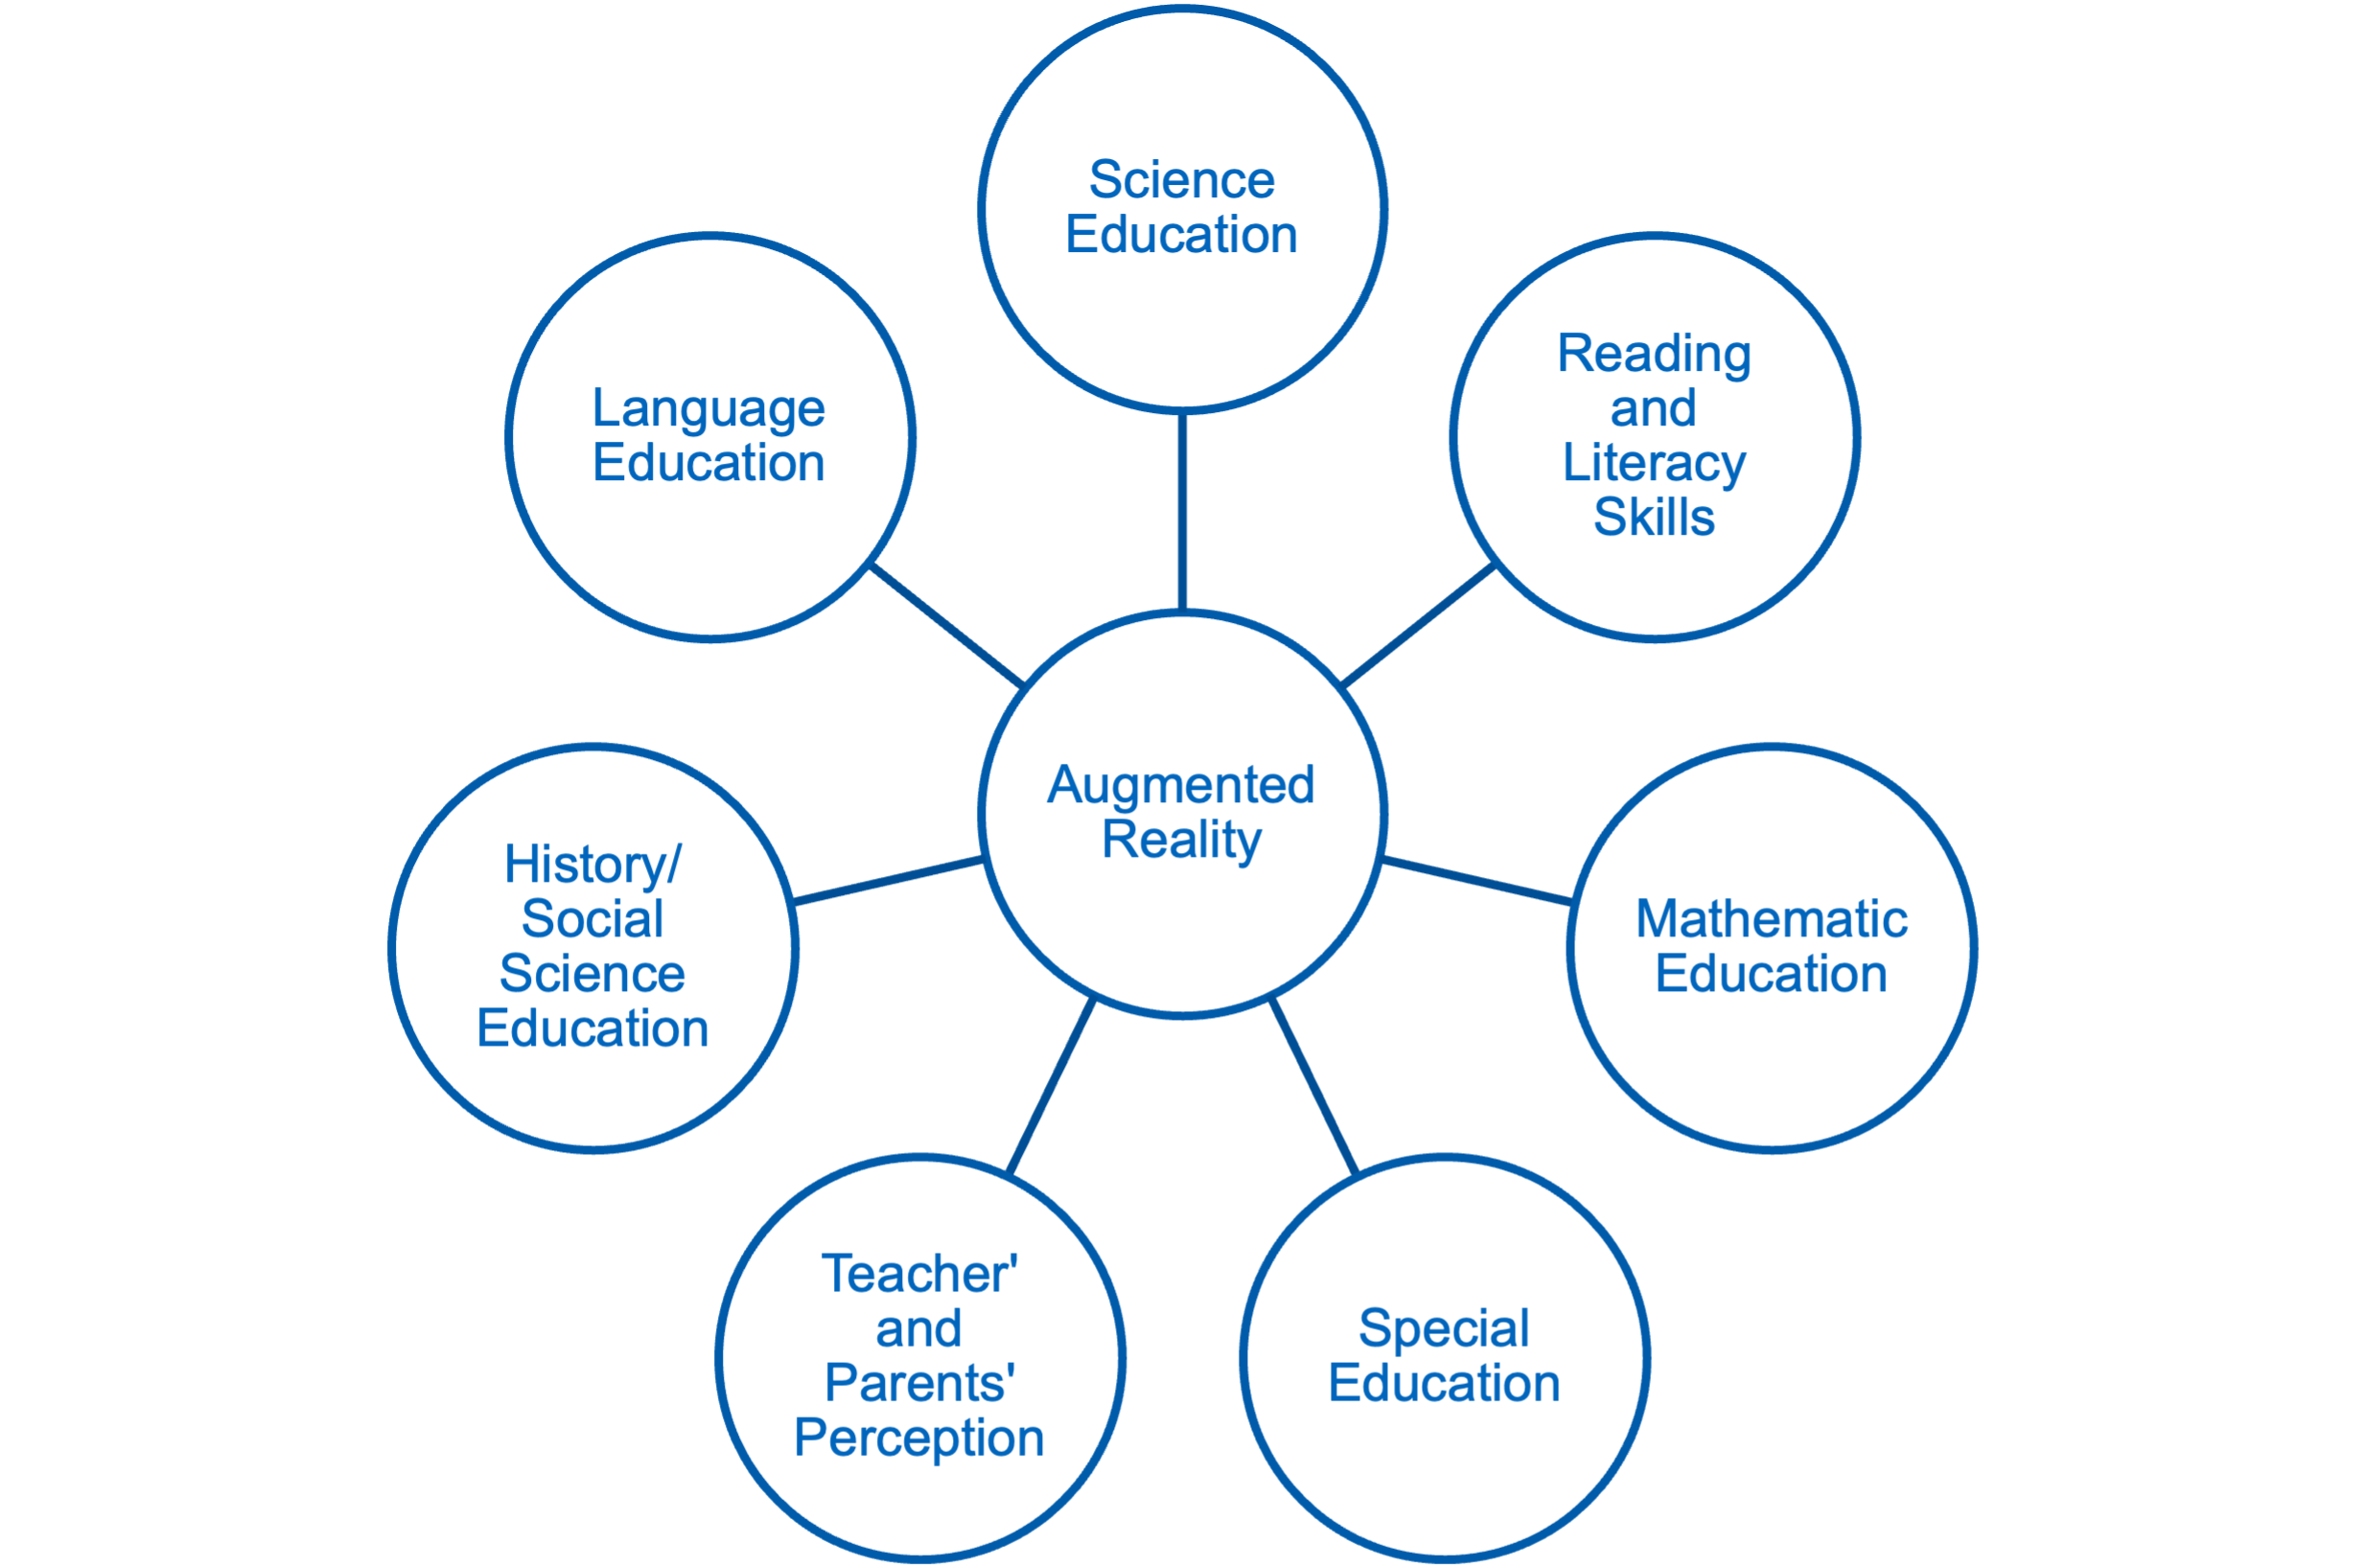
\includegraphics[scale=0.3]{img/sections.png}}
    \caption{Sektionen der Bildung \cite{b4}}
    \label{fig2}
\end{figure}

Während 5 dieser Sektionen mit den traditionellen Bildungsbereichen der Schulsysteme einhergeht, sind 
auch Themen wie Special Education (Bildung für Menschen mit Lernbehinderungen), sowie die Auswirkungen
und möglichen Ergebnisse der Anwendung und wie die Wahrnehmung der Lehrkräfte und Eltern ist, relevant.

\subsection{Primär und Sekundär}
Im folgenden wird die mögliche Anwendung von AR in den primären und sekundären Bildungsstuffen behandelt.
Desweiteren ist zu Bemerken, dass mit ''K-12 Education'' (Begriff aus dem angloamerikanischem Raum) der Abschnitt
von der Grundschule bis inklusive Sekundarstufe 1 beziehungsweise 2 gemeint ist. Die Integration von modernen AR
Technologien ermöglicht vielseitige Möglichkeiten, den Unterricht und das Lernen zu revolutionieren und zu bereichern.

Die Anwendung von AR in der Grundbildung ist vor allem in Richtung ''Gamification'', 
also den spielerischen Ansätzen in Lernkontexten, um möglicherweise die Motivation und das Engagement von Schülerinnen
und Schülern zu steigern. Augmented Reality kann es ermöglichen, sehr abstrakte und komplexe Lerninhalte durch interaktivere
Erlebnisse für junge Schüler zugänglicher zu machen. Beispielsweise können vorallem einige mathematische Konzepte,
die oftmals schwer verständlicher sind, durch Spiele und Simulationen visualisiert und dargestellt werden. Dadurch können
neben den zu erwartenden Lernefolgen auch das kreative Denken fördern.

Vor allem in den Naturwissenschaften kann AR eine innovative Möglichkeit sein, unterschiedliche Konzepte darzustellen.
Anwendungen können molekulare Strukturen, phsyikalische Phänome oder biologische Prozesse in interaktiven Umgebungen 
darstellen, die weitaus effektiver sind, als herkömmliche Lernmethoden. Darunter können vor allem Themen wie der Aufbau
von Antomen oder die Funktionsweise und Aufbau des Nervensystems fallen. Dadurch können Lernende diese Konzepte nicht nur sehen,
sondern auch damit interagieren und erforschen.\cite{b6}

Des weiteren können Anwendungen in der Augemented Reality für Projektarbeiten genutzt werden, in denen in einer kooperativen
und interaktive Lernumgebung Schülerinnen und Schüler gemeinsam digitale Modelle erstellen, erkunden und bearbeiten können.
Diese können dann den Mitschülern interaktiv präsentiert werden. Dies fördert nicht nur das Verständnis der gelehrten Inhalte,
sondern auch wichtige soziale Fähigkeiten, Kommunikation und Problemlösungsfähigkeiten.

\subsubsection*{Fallstudie}
Eine Fallstudie, welche eine Mögliche Anwendung von AR im primären Bildungssektor untersucht hat ist die Anwendung ''Cooking Math''.
Diese wurde an einer griechischen Grundschule testweise in den das grieschische Curriculum für Mathematik eingebaut und von einer Gruppe von
Pädagogikstudenten und Ingenieursstudenten durchgeführt.
Die Anwendung erlaubt es den Schülerinnen und Schülern mithilfe eines Tablets verschiedene mathematische Konzepte und Aufgaben zu
verstehen. Sinn ist es, mithilfe von ''Kochaufgaben'' (Abb. \ref{fig3}) einfache Aufgaben in Themen der Geometrie, den rationalen Zahlen und Gleichungen
zu untersuchen und zu lösen.

\begin{figure}[htbp]
    \centerline{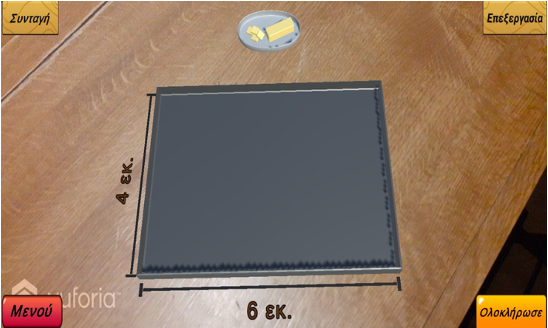
\includegraphics[scale=0.7]{img/geometrie.png}}
    \caption{Aufgabe im Bereich Geometrie}
    \label{fig3}
\end{figure}

Die Ergebnisse der System Usability Scale (SUS) Fragebögen und Interviews waren überwiegend positiv. Die Schüler zeigten Begeisterung, während 
der pdagogische Wert untersucht und Verbesserungen vorgeschlagen wurden. \cite{b8}

\subsection{Hochschule}
Die Anwendung von AR im Hochschulsektor bietet viele, weitreichende Möglichkeiten. Die Technologien können auch in diesem Sektor die traditionellen
Lernmethoden erweitern und interaktivere Auseinandersetzungen mit komplexen Konzepten ermöglichen.

\section{Weiterbildung}
TODO

\section{Potential}
TODO

\section{Fazit}
TODO

\begin{thebibliography}{00}
\bibitem{b1}  M. Dunleavy, C. Dede, and R. Mitchell, "Affordances and Limitations of Immersive Participatory Augmented Reality Simulations for Teaching and Learning". Journal of Science Education and Technology, 2009.
\bibitem{b2} M. E. C. Santos, A. Chen, T. Taketomi, G. Yamamoto, J .Miyazaki, and H. Kato, "Augmented Reality Learning Experiences: Survey of Prototype
Design and Evaluation". IEEE Transactions on Learning Technologies, 2014.
\bibitem{b3} J. Bacca, S. Baldiris, R. Fabregat, S. Graf, and Kinshuk, "Augmented Reality Trends in Education: A Systematic Review of Research and Applications". Educational Technology and Society, 2014.
\bibitem{b4} H. Cetin, “A Systematic Review of Studies on Augmented Reality Based Applications in Primary Education”, IJELS, 2022.
\bibitem{b5} J. Zhang, G. Li, Q. Huang, Q. Feng and H. Luo, „Augmented Reality in K–12 Education A Systematic Review and Meta-Analysis of the Literature from 2000 to 2020”, MDPI, 2022.
\bibitem{b6} M. Akçayır, and G. Akçayır, "Advantages and challenges associated with augmented reality for education: A systematic review of the literature". Educational Research Review, 2017.
\bibitem{b7} P. Chen, X. Liu, W. Cheng and R. Huang, "A review of using augmented reality in education from 2011 to 2016". Innovations in Smart Learning, 2017.
\bibitem{b8} C. Volioti, O. Christos, T. Sapounidis, G. Trachanas and E. Keramopoulos, "Augmented Reality in Primary Education: An Active Learning Approach in Mathematics", Computers, 2023.
\bibitem[w1]{w1} \href{https://www.cospaces.io/tech-check-ar-with-smartphones}{https://www.cospaces.io/tech-check-ar-with-smartphones} letzter Zugriff 07.07.2024 16:32
\bibitem[w2]{w2} \href{https://www.marketresearchfuture.com/reports/ar-vr-in-education-market-10834}{https://www.marketresearchfuture.com/reports/ar-vr-in-education-market-10834} letzter Zugriff 03.07.2024 20:38
\end{thebibliography}
\vspace{12pt}

\end{document}
